\documentclass{article}
\usepackage[utf8]{inputenc}

\title{EE2703 Applied Programming Lab \\ Assignment 7}
\author{
  \textbf{Name}: Neham Hitesh Jain\\
  \textbf{Roll Number}: EE19B084
}\date{April 15, 2021}

\usepackage{listings}
\usepackage{natbib}
\usepackage{geometry} % Used to adjust the document margins
\usepackage{amsmath}
\usepackage{color}
\usepackage{graphicx}
\definecolor{dkgreen}{rgb}{0,0.6,0}
\definecolor{gray}{rgb}{0.5,0.5,0.5}
\definecolor{mauve}{rgb}{0.58,0,0.82}

\lstset{frame=tb,
  language=Python,
  aboveskip=3mm,
  belowskip=3mm,
  showstringspaces=false,
  columns=flexible,
  basicstyle={\small\ttfamily},
  numbers=none,
  numberstyle=\tiny\color{gray},
  keywordstyle=\color{blue},
  commentstyle=\color{dkgreen},
  stringstyle=\color{mauve},
  breaklines=true,
  breakatwhitespace=true,
  tabsize=3
}

\geometry{verbose,tmargin=1in,bmargin=1in,lmargin=1.5in,rmargin=1.5in}

\begin{document}

\maketitle
\newpage

\begin{abstract}

In this assignment, we deal with Linear Time Invariant systems and their
responses to certain inputs. We use the scipy.signal module to perform
analysis of systems with rational polynomial transfer functions. We look
at a coupled system of differential equations, and also a linear
electrical circuit which behaves like a low-pass filter.

\end{abstract}

\section*{Question 1,2}\label{question-1}

We solve for the response by using the property that the Laplace
transform of the output \(X(s)\) of a system with transfer function
\(H(s)\) to an input with Laplace transform \(F(s)\) is given by:

\[X(s) = H(s) F(s)\]

\noindent
We are given an equation describing forced oscillatory system (with zero initial conditions) as:

\begin{equation}
    \ddot x + 2.25x = f(t)
\end{equation}

where $x$ is the output and $f(t)$ is the input.
\\

\noindent
Thus the transfer function of the system is given by:

\begin{equation}
   H(s) = \frac{1}{s^2+2.25}
\end{equation}
\\
Now, we are given input f(t) as $cos(1.5t)e^{-0.5t}u_0(t)$ i.e.
\begin{equation}
   F(s) = \frac{s+0.5}{(s+0.5)^2+2.25}
\end{equation}
\\
\noindent
Thus the output will be $X(s) = H(s)F(s)$
\begin{equation}
   X(s) = \frac{s+0.5}{((s+0.5)^2+2.25)(s^2+2.25)}
\end{equation}
\\
\noindent
We then use the sp.impulse function to find the inverse Laplace
transform of the output over a certain range of times:


\begin{lstlisting}

def input_signal_laplace(freq,decay):
    """Transfer function of the given system"""
    
    n = np.poly1d([1,decay])
    d = n*n+freq**2
    return n,d

def general_transfer_fcn(wn=1.5,zeta=0,gain=1/2.25):
    """General transfer function for a second order system"""
    
    n = np.poly1d([wn**2*gain])
    d = np.poly1d([1,2*wn*zeta,wn**2])
    return n,d

def lti_solver(decay,freq=1.5):
    """Find the response to the given system to a decaying cosine."""
    
    input_numerator, input_denominator = input_signal_laplace(freq,decay=decay)
    transfer_numerator, transfer_denominator = general_transfer_fcn()

    output_numerator,output_denominator = input_numerator*transfer_numerator, input_denominator*transfer_denominator
    out_s = sp.lti(output_numerator.coeffs, output_denominator.coeffs)

    t = np.linspace(0,50,1000)
    
    return sp.impulse(out_s,None,t)

\end{lstlisting}

\begin{figure}[tbh!]
\centering
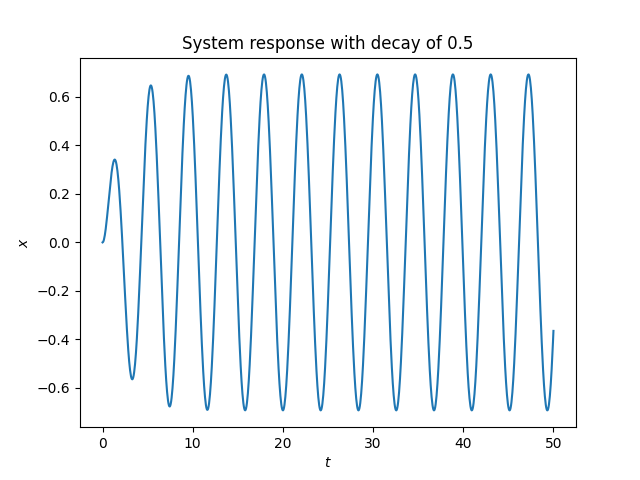
\includegraphics[scale=0.6]{plots/System response with decay of 0.5.png}
\caption{System Response with Decay = 0.5}
\label{fig:System Response with Decay = 0.5}
\end{figure}

\begin{figure}[tbh!]
\centering
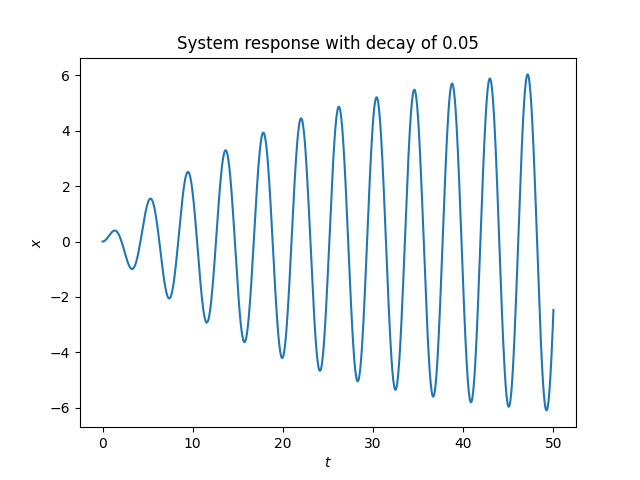
\includegraphics[scale=0.6]{plots/System response with decay of 0.05.png}
\caption{System Response with Decay = 0.05}
\label{fig:System Response with Decay = 0.05}
\end{figure}
\newpage
We observe that the steady state response follows the same trend as the
previous case, except that it has a much larger amplitude. This is
because the input excited the system for a longer duration due to its
smaller decay constant. This resulted in a larger buildup of output due
to resonance. We can see that, during the buildup of the output, the
amplitude grows linearly. This is characteristic of resonance in a
second order system. This will be made clear by exciting the system with
slightly different frequencies:


\section*{Question 3}\label{Question 3}

We simulate the above equation but with varying frequencies this time.
\\

\begin{lstlisting}
#Question 3
transfer_fcn=general_transfer_fcn(wn=1.5,zeta=0,gain=1/2.25)
outs = []

def input_signal_time(t,decay=0.5,freq=1.5):
    """Exponentially decaying cosine function."""

    u_t = 1*(t>0)
    return np.cos(freq*t)*np.exp(-decay*t) * u_t

# List of frequencies to iterate over
freqs = np.linspace(1.4,1.6,5)
t = np.linspace(0,70,1000)
for freq in freqs:
    # solve
    t,y,_ = sp.lsim(transfer_fcn,input_signal_time(t,decay=0.05,freq=freq),t)
    # Store
    outs.append(y)

\end{lstlisting}

\noindent
The response is plotted for frequencies around \(1.5\):
\\
\begin{figure}[tbh!]
    \centering
    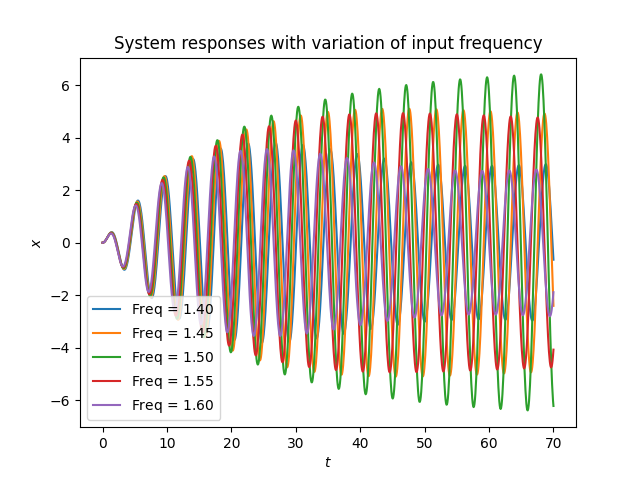
\includegraphics[scale=0.6]{plots/System responses with variation of input frequency.png}
    \caption{System Response with Frequencies around \(1.5\)}
    \label{fig:System Response with Frequencies around 1.5}
\end{figure}    
\newpage
We observe that an input with frequency of exactly \(1.5\) reaches the
largest steady state amplitude. This is because of the  resonance condition. 
Nearby frequencies are not tuned to the natural response of
the system, so their amplitudes die down after the initial rise before
reaching a steady state. This can also be understood by looking at the
magnitude of the transfer function at these frequencies.
\\ \\
We now look at the Bode Plot of the above transfer function: 
\\
\begin{figure}[tbh!]
    \centering
    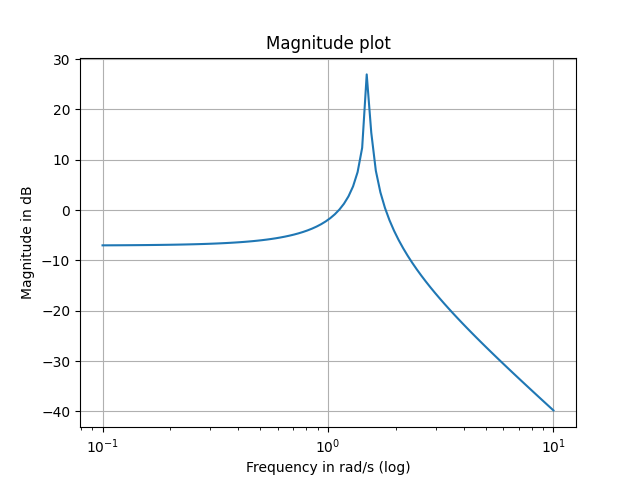
\includegraphics[scale=0.6]{plots/Magnitude plot.png}
    \caption{Magnitude Plot of Transfer Function in dB}
    \label{fig:Magnitude Plot 1}
\end{figure}

\begin{figure}[tbh!]
    \centering
    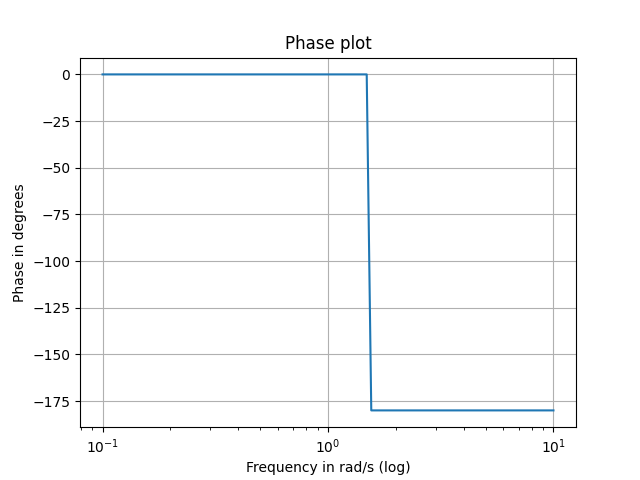
\includegraphics[scale=0.6]{plots/Phase plot.png}
    \caption{Phase Plot of Transfer Function}
    \label{fig:Phase Plot 1}
\end{figure}


\section*{Question 4}\label{Question 4}

We now consider a Coupled Differential System of Equations

\begin{equation}
    \ddot x + (x-y) = 0
\end{equation}

and 

\begin{equation}
    \ddot y + 2(y-x) = 0
\end{equation}

\noindent
With the initial conditions: $\dot x(0) =0,\dot y(0) =0,x(0) =1,y(0) =0$.
\\ \\
\noindent
Taking Laplace Transform and solving for $X(s)$ and $Y(s)$, We get:
\begin{equation}
    X(s) = \frac{s^2+2}{s^3 + 3s}
\end{equation}
\begin{equation}
    Y(s) = \frac{2}{s^3 + 3s}
\end{equation}
\\
Thus in Laplace Domain both equations are uncoupled. We now find the corresponding equations in time domain

\begin{lstlisting}
#Question 4
X_s = sp.lti([1,0,2],[1,0,3,0])
Y_s = sp.lti([2],[1,0,3,0])

t = np.linspace(0,20,1000)
t, x = sp.impulse(X_s,None,t)
t, y = sp.impulse(Y_s,None,t)

p6 = General_Plotter(r"$t$","Displacement","Responses of coupled system")
p6.general_plot(t,np.array([x,y]).T,legend_txt=[r"$x(t)$", r"$y(t)$"])
\end{lstlisting}

\begin{figure}[h!]
\centering
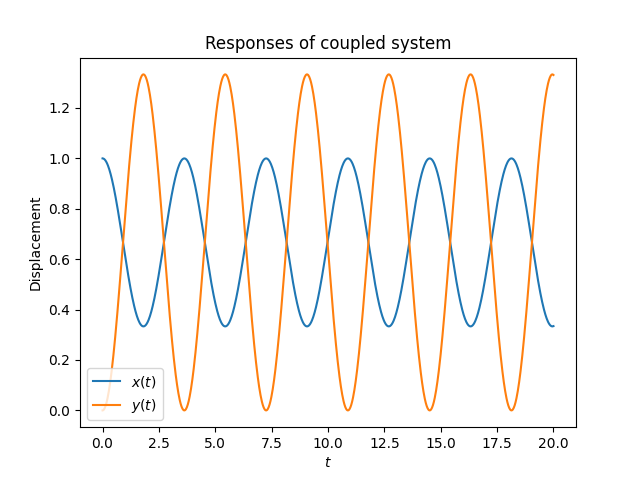
\includegraphics[scale=0.6]{plots/Responses of coupled system.png}
\caption{Displacement vs Time}
\label{Displacement X vs Time}
\end{figure}
\newpage

\begin{itemize}
    \item
      We observe that the solutions are sinusoidal with a certain DC offset.
    \item
      This is evident from the expressions of the Laplace Transforms of the
      solutions as the denominator contains a factor of \(s\).
    \item
      We observe that these two DC offsets are the same for both \(x\) and
      \(y\).
    \item
      They also oscillate with the same frequencies because the coefficient
      of the second derivative term is the same in both differential
      equations.
    
    \item
      The phase difference between \(x\) and \(y\) is 180 degrees.
      


    \item
      This system of equations models two masses attached to the two ends of
      an ideal spring with no damping. \(x\) and \(y\) are the positions of
      the masses in a reference frame moving at the same speed as the centre
      of mass, but offset from the centre of mass by some amount.
    
    \end{itemize}

\section*{Question 5}\label{Question-5}

We find the transfer function by finding the natural frequency and the
damping constant of the circuit. We then plot the Bode Plot of the given transfer
function.

\begin{lstlisting}
# Find the transfer function of the given circuit
R = 100
L = 1e-6
C = 1e-6

wn = 1/np.sqrt(L*C) # natural frequency
Q = 1/R * np.sqrt(L/C) # quality factor
zeta = 1/(2*Q) # damping constant

# transfer function
n,d = general_transfer_fcn(gain=1,wn=wn,zeta=zeta)
# make system
H = sp.lti(n,d)

# get bode plots
w,S,phi=H.bode()

p7 = General_Plotter("Frequency in rad/s (log)","Magnitude in dB","Magnitude plot 2")
p7.semilogx(w,S)

p8 = General_Plotter("Frequency in rad/s (log)","Phase in degrees","Phase plot 2")
p8.semilogx(w,phi)

\end{lstlisting}
    
\begin{figure}[h!]
    \centering
    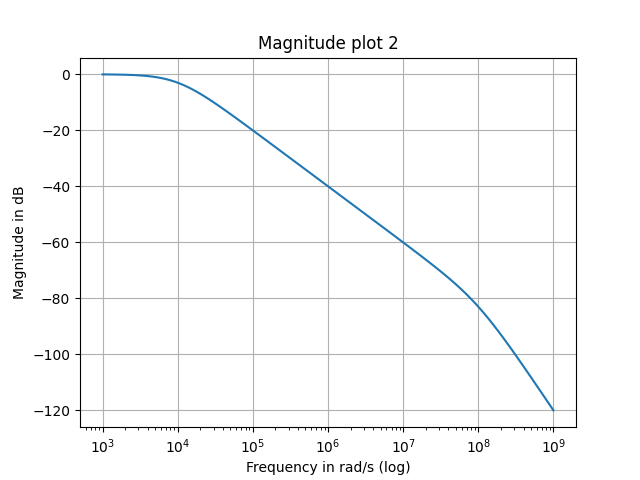
\includegraphics[scale=0.6]{plots/Magnitude plot 2.png}
    \caption{Magnitude Plot of Transfer Function in dB}
    \label{Magnitude Plot 2}
\end{figure}

\begin{figure}[h!]
    \centering
    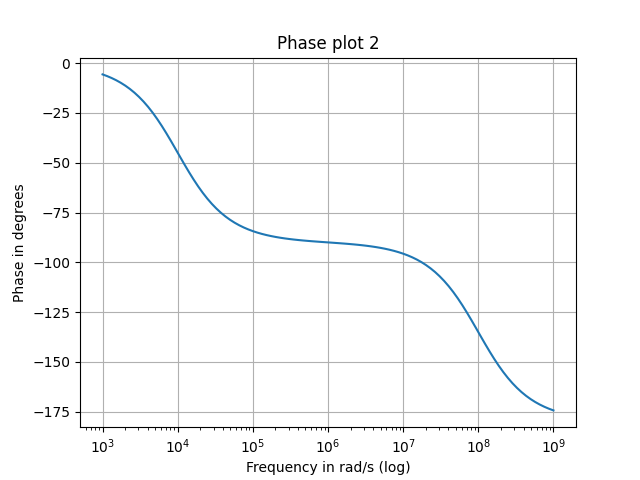
\includegraphics[scale=0.6]{plots/Phase plot 2.png}
    \caption{Phase Plot of Transfer Function}
    \label{Phase Plot 2}
\end{figure}
\newpage    
\begin{itemize}
    \item
      It is clear that there are two poles, one at around \(10^4\) rad/s and
      another at around \(10^8\) rad/s.
    \item
      Since the two poles are quite far apart, we can approximate the 3-dB
      bandwidth of the filter to be at the first pole, i.e., \(10^4\) rad/s.
    \item
      We therefore expect the system to pass frequencies lower than \(10^4\)
      rad/s and attenuate higher frequencies. We see this effect in the next
      part.
\end{itemize}
\newpage
\section*{Question 6}\label{Question-6}

We excite the system in Question 5 with two sinusoids, one whose
frequency is below the 3-dB bandwith and one whose frequency is higher.
\\
\begin{lstlisting}
# Transient Response
t1=np.linspace(0,30e-6,1000)
t1,y1,_ = sp.lsim(H,cosines(t1),t1)

# Steady State Response
t2=np.linspace(0,10e-3,1000)
t2,y2,_ = sp.lsim(H,cosines(t2),t2)

p9=General_Plotter(r"$t$ (sec)",r"$v_0(t)$",r"Response for 30 micro seconds")
p9.general_plot(t1,y1)


p10=General_Plotter(r"$t$ (sec)",r"$v_0(t)$",r"Response for 10 msec")
p10.general_plot(t2,y2)
\end{lstlisting}
    

We plot the time domain response in two parts, one for the first 30
\(\mu s\), to observe transient effects, and one for \(10\) msec, to
observe the steady state response.

\begin{figure}[tbh!]
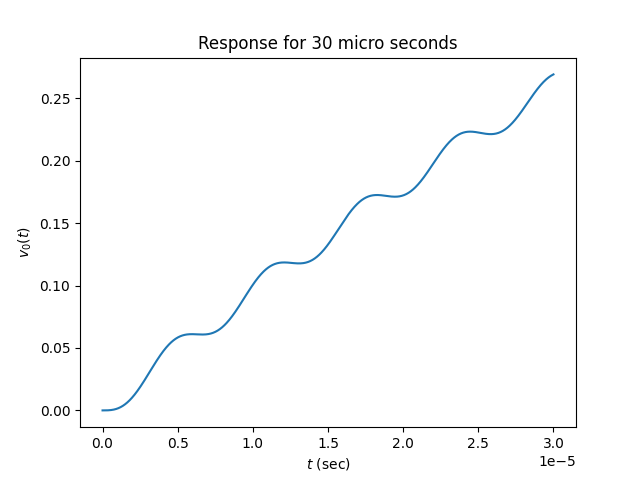
\includegraphics[scale=0.6]{plots/Response for 30 micro seconds.png}
\centering
\caption{System response for t$<$30us}
\label{fig:System response for t<30us}
\end{figure}
\clearpage
\begin{figure}[tbh!]
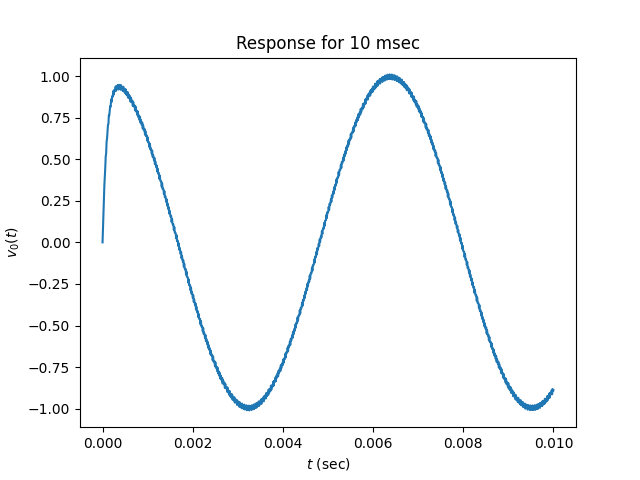
\includegraphics[scale=0.6]{plots/Response for 10 msec.png}
\centering
\caption{System response for t$<$10ms}
\label{fig:System response for t<10ms}
\end{figure}

\begin{itemize}
    
    \item
      The transient response of the system is rapidly increasing. This is
      because the system has to charge up to match the input amplitude. This
      results in a phase difference between the input and the output. This
      can also be interpreted as a delay between the input and the output
      signals.
    \item
      The response can be broken up into a low frequency component and a
      high frequency one, after the transient effect has died down.
    \item
      The high frequency component is extremely attenuated (by -40 dB
      infact), so in the 10 msec plot, it is almost not visible.
    \item
      The low frequency component passes through almost unaffected with an
      amplitude of slightly less than 1. This is because its frequency is
      below the 3-dB bandwidth of the system.
    \item
      Thus, it is clear that the system behaves like a low-pass filter.

\end{itemize}
    
\newpage
\section*{Conclusion}
We used the scipy.signal library to solve circuits and equations in Laplace Domain including forced response of simple spring body system, 
a coupled spring problem and a low-pass filter circuit was analysed and output signal found for a mixed frequency input signal.

\end{document}
